\documentclass{../source/Experiment}

\major{信息工程}
\name{姚桂涛}
\title{基于RV32I指令集的RISC-V微处理器设计}
\stuid{3190105597}
\college{信息与电子工程学院}
\date{\today}
\lab{教11-400}
\course{计算机组成与设计}
\instructor{屈民军、唐奕}
\grades{}
\expname{RISC-V微处理器设计}
\exptype{设计验证}
\partner{}
\begin{document}
    \makecover
    \makeheader
    \section{实验目的}
    
    \section{实验任务}
        \subsection{基本要求}
        设计一个流水线RISC-V微处理器,具体要求如下所述。

        (1) \, 至少运行下列RV32I核心指令。

        算术运算指令:add、sub、addi

        逻辑运算指令:and、or、xor、slt、sltu、di、ori、xori、slti、sltiu

        移位指令:sll、srl、sra、slli、srli、srai

        条件分支指令:beq、bne、blt、bge、bltu、eu

        无条件跳转指令:jal、jalr

        数据传送指令:lw、sw、lui、auipc
    
        空指令:nop

        (2) \, 采用 5 级流水线技术,对数据冒险实现转发或阻塞功能。

        (3) \, 在 Nexys Video 开发系统中实现RISC-V 微处理器, 要求 CPU 的运行速度大于 25MHz。
        \subsection{扩展要求}
        (1) \, 要求设计的微处理器还能运行lb、lh、ld、lbu、lhu、lwu、sb、sh 或 sd 等字节、半字和双字数据传送指令。

        (2) \, 要求设计的CPU 增加异常(exception)、自陷(trap)、中断(interrupt)等处理方案。
        
    \section{实验原理与模块设计}
        \subsection{总体设计}
        流水线是数字系统中一种提高系统稳定性和工作速度的方法,广泛应用于高档CPU 的架构中。根据RISC-V 处理器指令的特点,将指令整体的处理过程分为取指令(IF)、指令译码(ID)、执行(EX)、存储器访问(MEM)和寄存器写回(WB)五级。如图30. 2 示,一个指令的执行需要 5 个时钟周期,每个时钟周期的上升沿来临时,此指令所代表的一系列数据和控制信息将转移到下一级处理。

        图  所示为符合设计要求的流水线 RISC-V 微处理器的原理框图,采用五级流水线。由于在流水线中 ,数据和控制信息将在时钟周期的上升沿转移到下一级,所以规定流水线转移的变量命名遵守如下 格式:名称\_流水线级名称。如,在 ID 级指令译码电路(decode)产生的寄存器写允许信号 RegWrite 在ID 级、EX 级、MEM 级和WB 级上的命名分别为RegWrite\_id、RegWrite\_ex 、RegWrite\_mem 和RegWrite\_wb。在顶层文件中,类似的变量名称有近百个,这样的命名方式起到了很好的识别作用。

        \subsection{流水线RISC-V微处理器的设计}
        根据流水线不同阶段,将系统划分为 IF、ID、EX 和 MEM 四大模块,WB 部分功能电路非常简单,可直接在顶层文件中设计。另外,系统还包含 IF/ID、ID/EX、EX/MEM、MEM/WB 四个流水线寄存器。
        \subsubsection{取指令级模块(IF)的设计}
        IF 模块由指令指针寄存器(PC)、指令存储器子模块(Instruction ROM)、指令指针选择器(MUX)
        和一个 32 位加法器组成,IF 模块接口信息如表  所示。

        核心代码如下:

        其中
        
        \subsubsection{指令译码模块(ID)的设计}
        指令译码模块的主要作用是从机器码中解析出指令,并根据解析结果输出各种控制信号。ID 模块主要
        由指令译码(Decode)、寄存器堆(Registers)、冒险检测、分支检测和加法器等组成。ID 模块的接口信息如表  所示。
        
        (1) \, 寄存器堆(Register)子模块的设计

        寄存器堆由 32 个 32 位寄存器组成,这些寄存器通过寄存器号进行读写存取。寄存器堆的原理框图如图30.8 所示。因为读取寄存器不会更改其内容,故只需提供寄存号即可读出该寄存器内容。读取端口采用数据选择器即可实现读取功能。

        寄存器堆设计还应解决三阶数据相关的数据转发问题。当满足三阶数据相关条件时,寄存器具有Read After Write 特性。

        RBW子模块核心代码如下:

        实现Read After Write寄存堆代码如下:

        (2) \, 指令译码(包含立即数产生电路)子模块的设计

        该子模块主要作用是根据指令确定各个控制信号的值,同时产生立即数 Imm 和偏移量offet。该模块是一个组合电路。

        根据操作数的来源和立即数的不同,将指令细分为不同类型,并对于不同类型产生不同的控制信号。同时产生立即数和偏移量。

        核心代码如下:

        (3) \, 分支检测电路的设计

        分支检测电路主要用于判断分支条件是否成立,在 Verilog HDL 可以用比较运算符号“>”、“==” 和“<”描述,但要注意符号数和无符号数的处理方法不同。在这里,我们用加法器来实现。

        用一个 32 位加法器完成rs1Data+(~rs2Data)+1(即 rs1Data-rs2Data),设结果为 sum [31:0] 。

        确定比较运算的结果。对于比较运算来说,如果最高位不同,即rs1Data [31]  rs2Data [31],可根据rs1Data [31]、rs2Data [31]决定比较结果,但是应注意符号数、无符号数的最高位rs1Data [31]、rs2Data [31] 代表意义不同。若两数最高位相同,则两数之差不会溢出,所以比较运算结果可由两个操作数之差的符号位 sum[31]决定。

        最终得到符号数与无符号数比较运算的结果:

        $ \rm isLT=rs1Data[31]\&\&(~rs2Data[31]) || (rs1Data[31]~^rs2Data[31]) \&\& sum[31]$

        $ \rm isLTU= (~rs1Data[31] )\&\& rs2Data[31] || (rs1Data[31]~^rs2Data[31]) \&\& sum[31]$

        最后用数据选择器完成下式即完成分支检测。

        $$Branch = \left\{
            \begin{aligned}
             & ~ (| sum[31 : 0]); & SB\_type & \, \& \& (funct3 == beq\_funct3 )\\
             & | sum[31 : 0];  & SB\_type & \, \& \& (funct3 = bne\_funct3 )\\
             & isLT;  & SB\_type & \, \& \&(funct3 = blt\_funct3 )\\
             & ~ isLT ;  & SB\_type & \, \& \& (funct3 = bge\_funct3 )\\
             & isLTU ;  & SB\_type & \, \& \& (funct3 = bltu\_funct 3)\\
             & ~ isLTU ;  & SB\_type & \, \& \& (funct3 = bgeu\_funct3)\\
             & 0  & others  & 
            \end{aligned}\right.   
        $$

        (4) \, 冒险检测功能电路(Hazard Detector)的设计

        由前面分析可知,冒险成立的条件为:

        上一条指令必须是lw 指令(MemRead\_ex=1);两条指令读写同一个寄存器(rdAddr\_ex=rs1Addr\_id 或 rdAddr\_ex=rs2Addr\_id)。

        当冒险成立应清空 ID/EX 寄存器并且阻塞流水线ID 级、IF 级流水线,所以有

        Stall=((rdAddr\_ex==rs1Addr\_id) || (rdAddr\_ex==rs2Addr\_id))\&\& MemRead\_ex

        IFWrite= ~Stall

        在用 VerilogHDL 描述ID 模块时,冒险检测功能电路(Hazard Detector)等功能单元比较简单,建议直接在ID 顶层描述。

        \subsubsection{执行模块(EX)的设计}
        执行模块主要由 ALU 子模块、数据前推电路( Forwarding)及若干数据选择器组成。执行模块的接口信息如表  所示。

        (1) \, ALU子模块的设计

        算术逻辑运算单元(ALU)提供 CPU 的基本运算能力,如加、减、与、或、比较、移位等。具体而言,ALU 输入为两个操作数A、B 和控制信号ALUCode,由控制信号ALUCode 决定采用何种运算,运算结果为 ALUResult。整理表 30.5 所示的ALUCode 的功能表,可得到ALU 的功能表,如表 所示。

        ALU核心代码如下:

        (2) \, 数据前推电路的设计

        操作数 A 和 B 分别由数据选择器决定,数据选择器地址信号 ForwardA、ForwardB 的含义如表 30.9所示。

        同时根据一、二阶数据相关判断条件,可以得到:

        
        \subsubsection{数据存储器模块(DataRAM)的设计}
        数据存储器可用Xilinx 的 IP 内核实现。考虑到 FPGA 的资源,数据存储器可设计为容量为 64×32 bit的单端口RAM,输出采用组合输出(Non Registered)。

        由于数据存储器容量为 64×32 bit,故存储器地址共 6 位,与ALUResult\_mem[7:2]连接。


        \subsubsection{流水线寄存器的设计}
        流水线寄存器负责将流水线的各部分分开,共有 IF/ID、ID/EX、EX/MEM、MEM/WB 四组,对四组
        流水线寄存器要求不完全相同,因此设计也有不同考虑。
        
        EX/MEM、MEM/WB 两组流水线寄存器只是普通的D 型寄存器。
        
        当流水线发生数据冒险时,需要清空 ID/EX 流水线寄存器而插入一个气泡,因此 ID/EX 流水线寄存
        器是一个带同步清零功能的D 型寄存器。
        
        当流水线发生数据冒险时,需要阻塞 IF/ID 流水线寄存器;若跳转指令或分支成立,则还需要清空
        ID/EX 流水线寄存器。因此,IF/ID 流水线寄存器除同步清零功能外,还需要具有保持功能(即具有使能
        EN 信号输入)。
        \subsubsection{顶层文件的设计}

        按照图 30.3 所示的原理框图连接各模块即可。为了测试方便,可将关键变量输出,关键变量有:指令指针PC、指令码 Instruction\_id、流水线插入气泡标志 Stall、分支标志 JumpFlag 即\{Jump, Branch\}、ALU 输入输出(ALU\_A、ALU\_B、ALUResult\_ex)和数据存储器的输出 MemDout\_mem。

        备注:具体代码过于长,具体可以参见solution中的代码源文件。

    \subsection{实验设备}
        \begin{enumerate}
            \item  装有Vivado 和 ModelSim SE 软件的计算机。
            \item  Nexys Video 开发板一套。
            \item  带有HDMI 接口的显示器一台。
        \end{enumerate}

    \section{实验结果}
        \subsection{Decode仿真}
            \subsubsection{仿真波形}
                \begin{figure}[H]
                    \centering
                    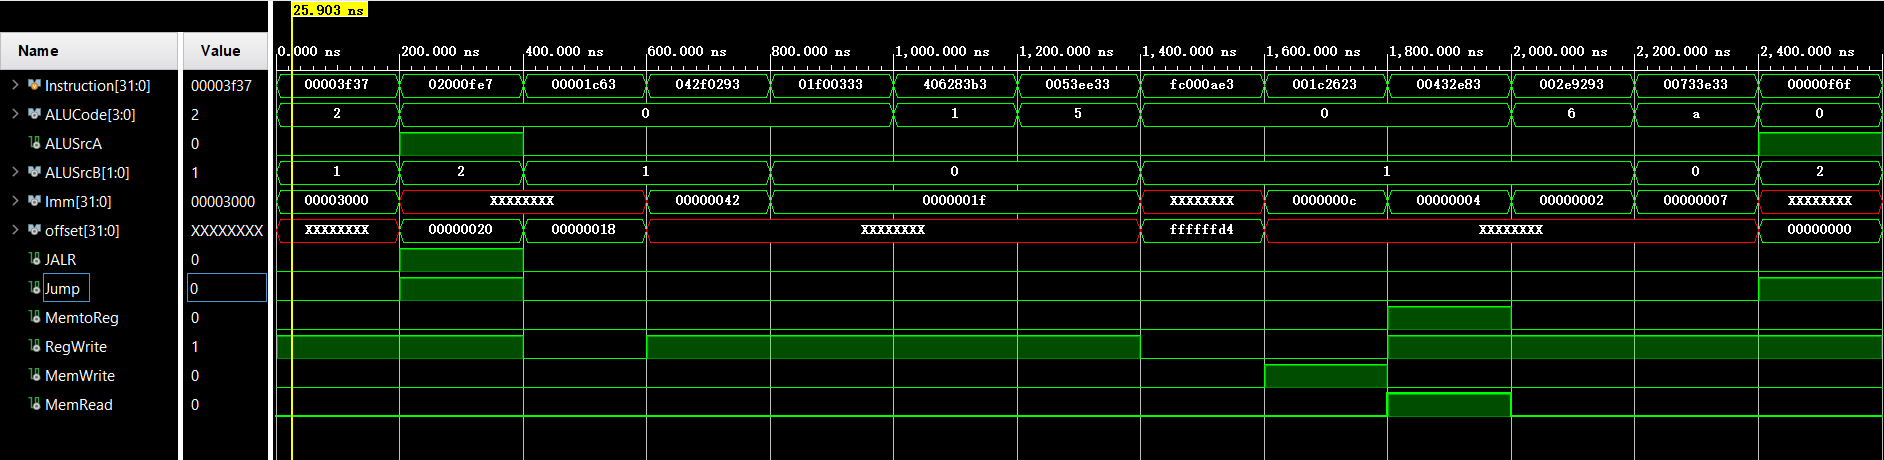
\includegraphics[width = 1\textwidth]{cpu_Decode_1}
                    \caption{Decode模块仿真波形图}
                \end{figure}
            \subsubsection{仿真结果}
                \begin{enumerate}
                    \item lui x30, 0x3000,为 U 型, Imm = 0x0000\_3000,offset 无意义,ALUCode=4’d2,ALUSrcA=0,ALUSrcB=2’b01,LUI 指令需要写回,RegWrite=1。
                    \item jalr X31, later(x0), I 型, Imm 无意义,offset=0x0000\_0020,ALUCode=4’d0,
                    ALUSrcA=1,ALUSrcB=2’b10,JALR=1,Jump=1,JALR 指令需要写回,RegWrite=1。
                    \item bne x0, x0, end, SB 型, Imm 无意义,offset=0x0000\_0018,ALUCode=4’d0,ALUSrcA=0,
                    ALUSrcB=2’b01,BNE 指令不需要写回,RegWrite=0。
                    \item addi x5, x30, 42, I型,Imm =0x0000\_0042,offset无意义,ALUCode=4’d0,ALUSrcA=0,
                    ALUSrcB=2’b01,ADDI 指令需要写回,RegWrite=1。
                    \item add x6, x0, x31, R 型, Imm 无意义,offset 无意义,ALUCode=4’d0,ALUSrcA=0,
                    ALUSrcB=2’b00,ADD 指令需要写回,RegWrite=1。
                    \item sub x7, x5, x6, R 型, Imm 无意义,offset 无意义,ALUCode=4’d1,ALUSrcA=0,
                    ALUSrcB=2’b00,SUB 指令需要写回,RegWrite=1。
                    \item or x28, x7, x5, R 型, Imm 无意义,offset 无意义,ALUCode=4’d5,ALUSrcA=0,
                    ALUSrcB=2’b00,OR 指令需要写回,RegWrite=1。
                    \item beq x0, x0, earlier, SB 型, Imm 无意义,offset=0xffff\_ffd4,ALUCode=4’d0,
                    ALUSrcA=0,ALUSrcB=2’b01,BEQ 指令不需要写回,RegWrite=0。
                    \item sw x28, 0C(x0), S 型, Imm =0x0000\_000c,offset 无意义,ALUCode=4’d0,ALUSrcA=0,ALUSrcB=2’b01,MemWrite=1。
                    \item lw x29, 04(x6), I 型, Imm =0x0000\_0004,offset 无意义,ALUCode=4’d0,ALUSrcA=0,ALUSrcB=2’b01,MemRead=1,MemtoReg=1,RegWrite=1。
                    \item sll x5, x29,2, I 型, Imm =0x0000\_0002,offset 无意义,ALUCode=4’d6,ALUSrcA=0,ALUSrcB=2’b01, RegWrite=1。
                    \item sltu x28, x6,x7, R 型, Imm 无意义,offset 无意义,ALUCode=4’d10,ALUSrcA=0,
                    ALUSrcB=2’b00, RegWrite=1。
                    \item jal x31, done, UJ 型, Imm 无意义,offset=0x0000\_0000,ALUCode=4’d1ALUSrcA=1,
                    ALUSrcB=2’b10,SUB 指令需要写回,RegWrite=1。
                \end{enumerate}

        \subsection{ALU模块仿真}
            \subsubsection{仿真波形}
                \begin{figure}[H]
                    \centering
                    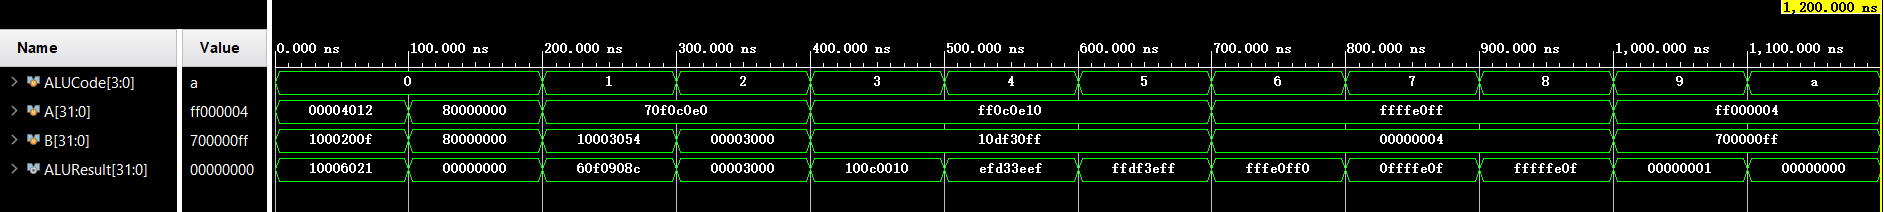
\includegraphics[width = 1\textwidth]{cpu_ALU_1}
                    \caption{ALU模块仿真波形图}
                \end{figure}               
            \subsubsection{仿真结果}
            从左到右对应的指令分别为:

            add ,\,  add ,\,  sub ,\,  lui ,\,  and ,\,  xor ,\,  or ,\,  sll ,\,  srl ,\,  sra ,\,  slt ,\,  sltu

            经过简单计算,结果正确。

        \subsection{IF模块仿真}
            \subsubsection{仿真波形}
                \begin{figure}[H]
                    \centering
                    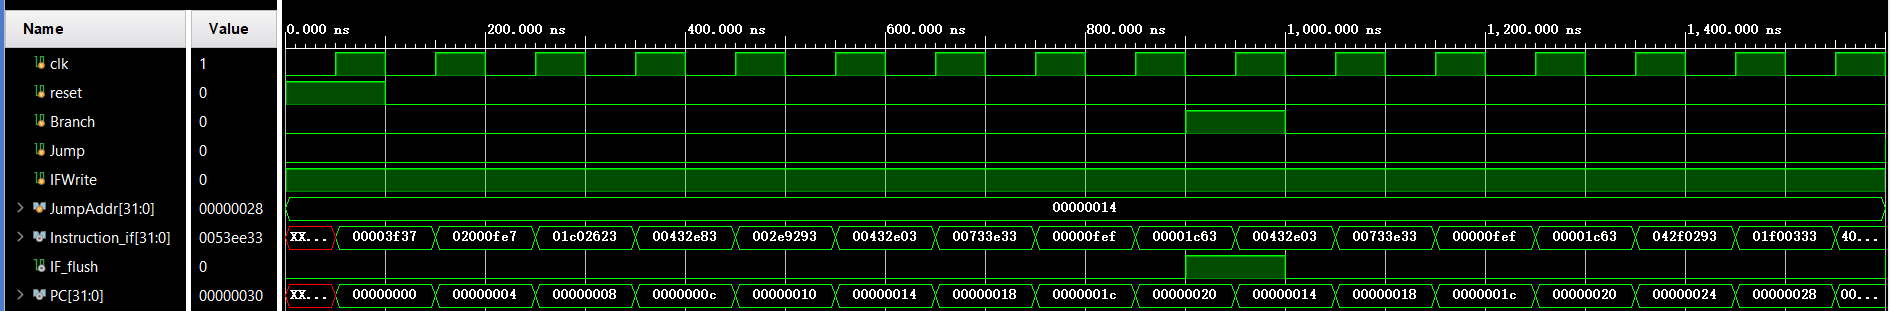
\includegraphics[width = 1\textwidth]{cpu_IF_1}
                    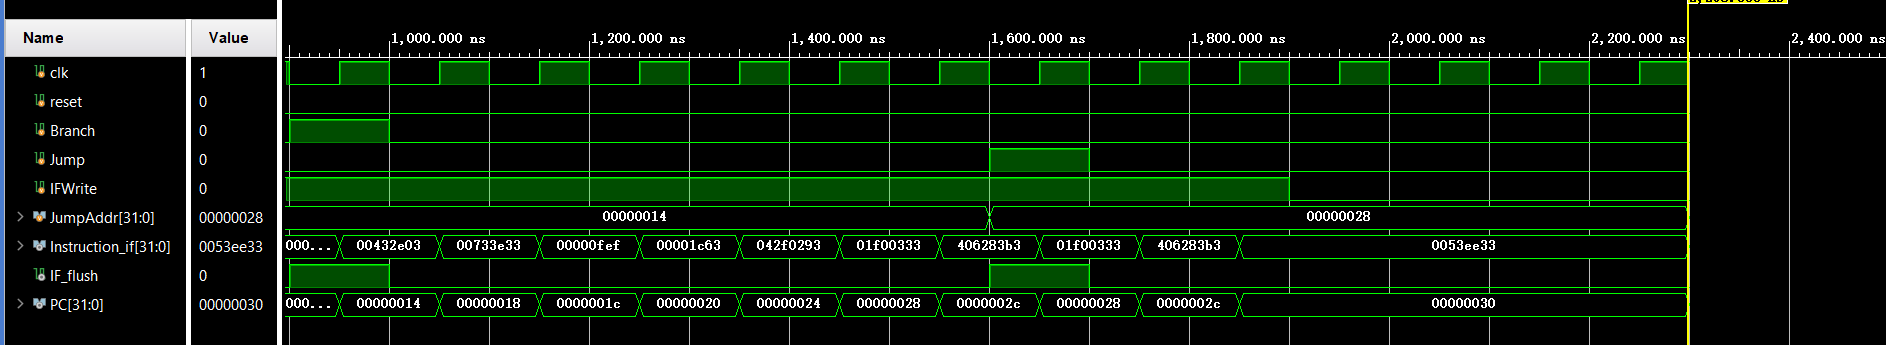
\includegraphics[width = 1\textwidth]{cpu_IF_2}
                    \caption{IF模块仿真波形图}
                \end{figure}    
            \subsubsection{仿真结果}
            从图中可以看出,当Branch与Jump都是0时,PC依次递增。当Branch或Jump为1时,PC可以实现正确的跳转。

        \subsection{顶层模块仿真}
            \subsubsection{仿真波形}
                \begin{figure}[H]
                    \centering
                    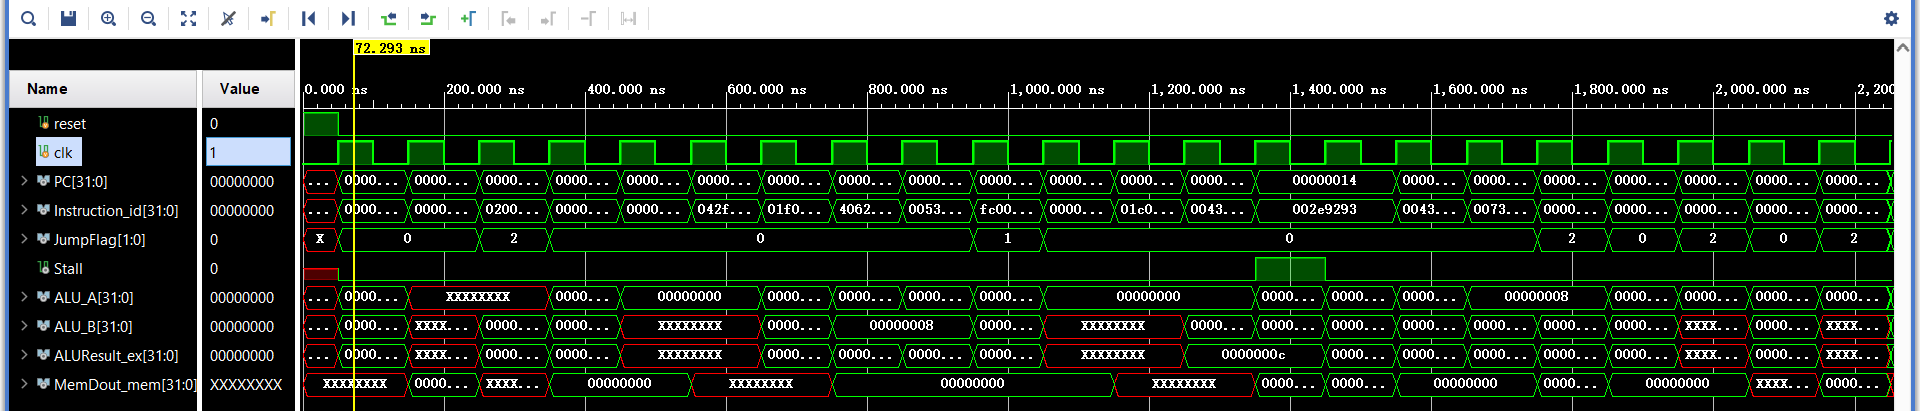
\includegraphics[width = 1\textwidth]{RiscV}
                    \caption{cpu模块仿真波形图}
                \end{figure} 
            \subsubsection{仿真结果}
            将仿真结果与下表比对正常。
        \subsection{上板验证}
            \begin{figure}
                \centering
                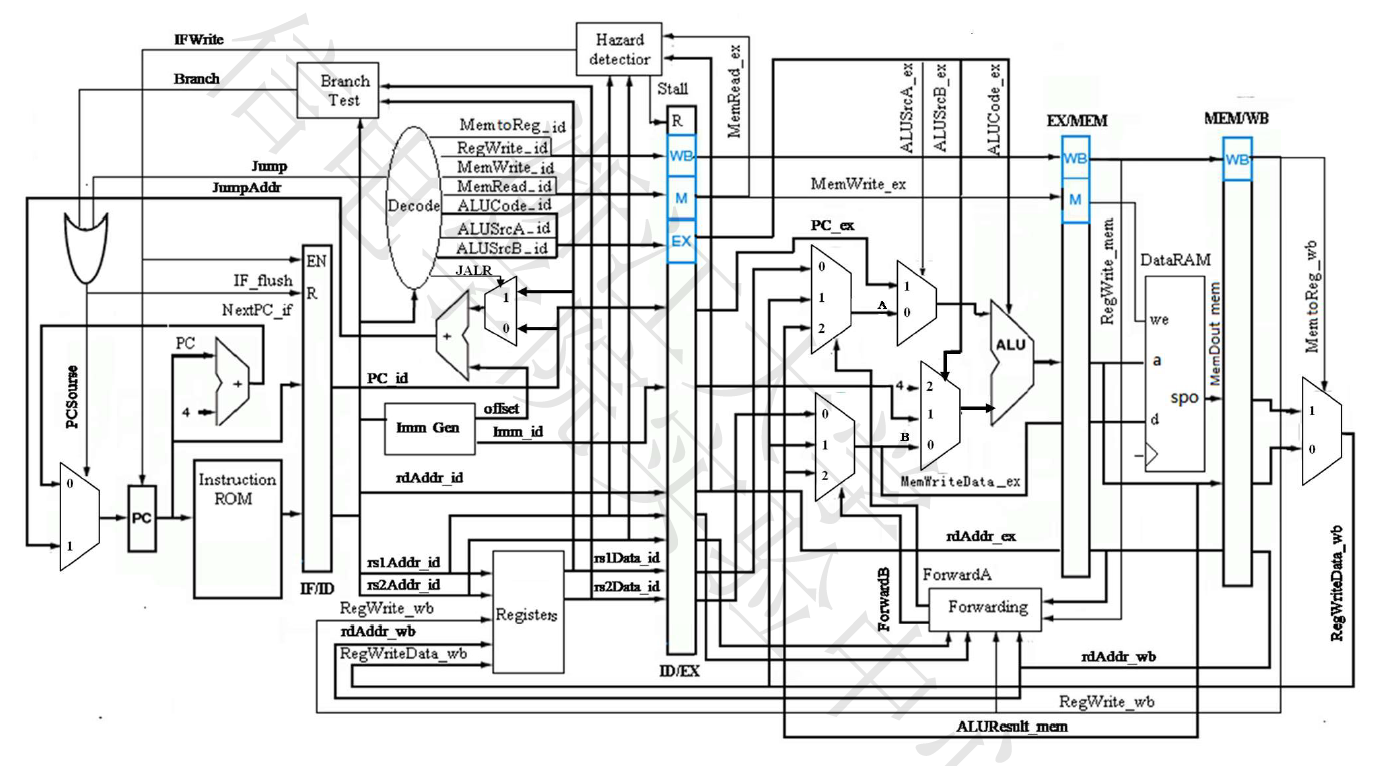
\includegraphics[width = 0.6\textwidth]{cpu.png}
                \caption{上板结果之一}
            \end{figure}
    \section{问题记录}
        \begin{enumerate}
            \item 刚开始实验的时候,看着实验指导书无从下手,难以理解整个CPU的架构。在听从老师的建议之后,我开始从一些比较简单或者实验指导书说明的比较详细的部分入手,开始写部分的实验代码。同时随着理论课程的学习,慢慢地对于各个部分的架构有了更加深刻的认识,而实验的进行也帮助我更加深刻地理解理论课学到的知识。
            \item 实验一个很大的难点是代码中有非常多的变量和传输线,所以很多时候容易漏掉或者看错一些端口。所以为了尽量减少这些问题,我尽量使代码的格式规范化,命名尽量和结构框架图中的一致,事实证明这样的习惯极大的帮助了我的调试。
            \item 在调试过程中,发现Decode模块的Imm和offset在应该是不确定的状态时(比如I型指令时offset应为不确定状态)却有着之前确定的状态,查看代码之后发现是在某些if语句下未给应该是不确定状态的Imm或offset赋值x。
            \item 在第15个时钟周期的时候,MemDout并没有出现正确的值,我开始一直在第15个周期的各个模块去查看相关的值是否正确,最后才意识到这里时stall之后的值,应去stall之前的那条指令去检查。
            \item 设计 ALU 的时候遇到 Binvert 位扩展的问题,最后通过百度解决了问题。
        \end{enumerate}

    \section{思考题}
    如下面两条指令,条件分支指令试图读取上一条指令的目标寄存器,插入气泡或数据转发都无法解决

    流水线冲突问题。为什么在大多CPU 架构中,都不去解决这一问题?这一问题应在什么层面中解决?
        
    lw X28, 04(X6)
    beq X28,x29,Loop

    答:插入一气泡,将 MEM/WB 寄存器的数据转发到 EX,这样似乎是可以的。经典的 MIPS Ⅰ使用了负载延迟槽,在 lw 后面加入 nop 但是负载延迟在硬件上非常不可预知,从 RAM 或缓存 load,可能会因资源竞争而变慢。负载延迟使延迟增加,因此大多数 CPU 架构中不去解决这一问题。后来的 MIPS 增加了死锁来避免填充 nop。

    这一问题主要靠汇编器调整指令顺序来解决


\end{document}